The Bode plot of the inner loop $P_{in}(s)$, and the loop gain with PD control $P_{in}(s)C_{PD}(s)$, are shown in Figure~\ref{fig:hw_ballbeam_bode_specs_in}.
\begin{figure}[H]
   \centering
   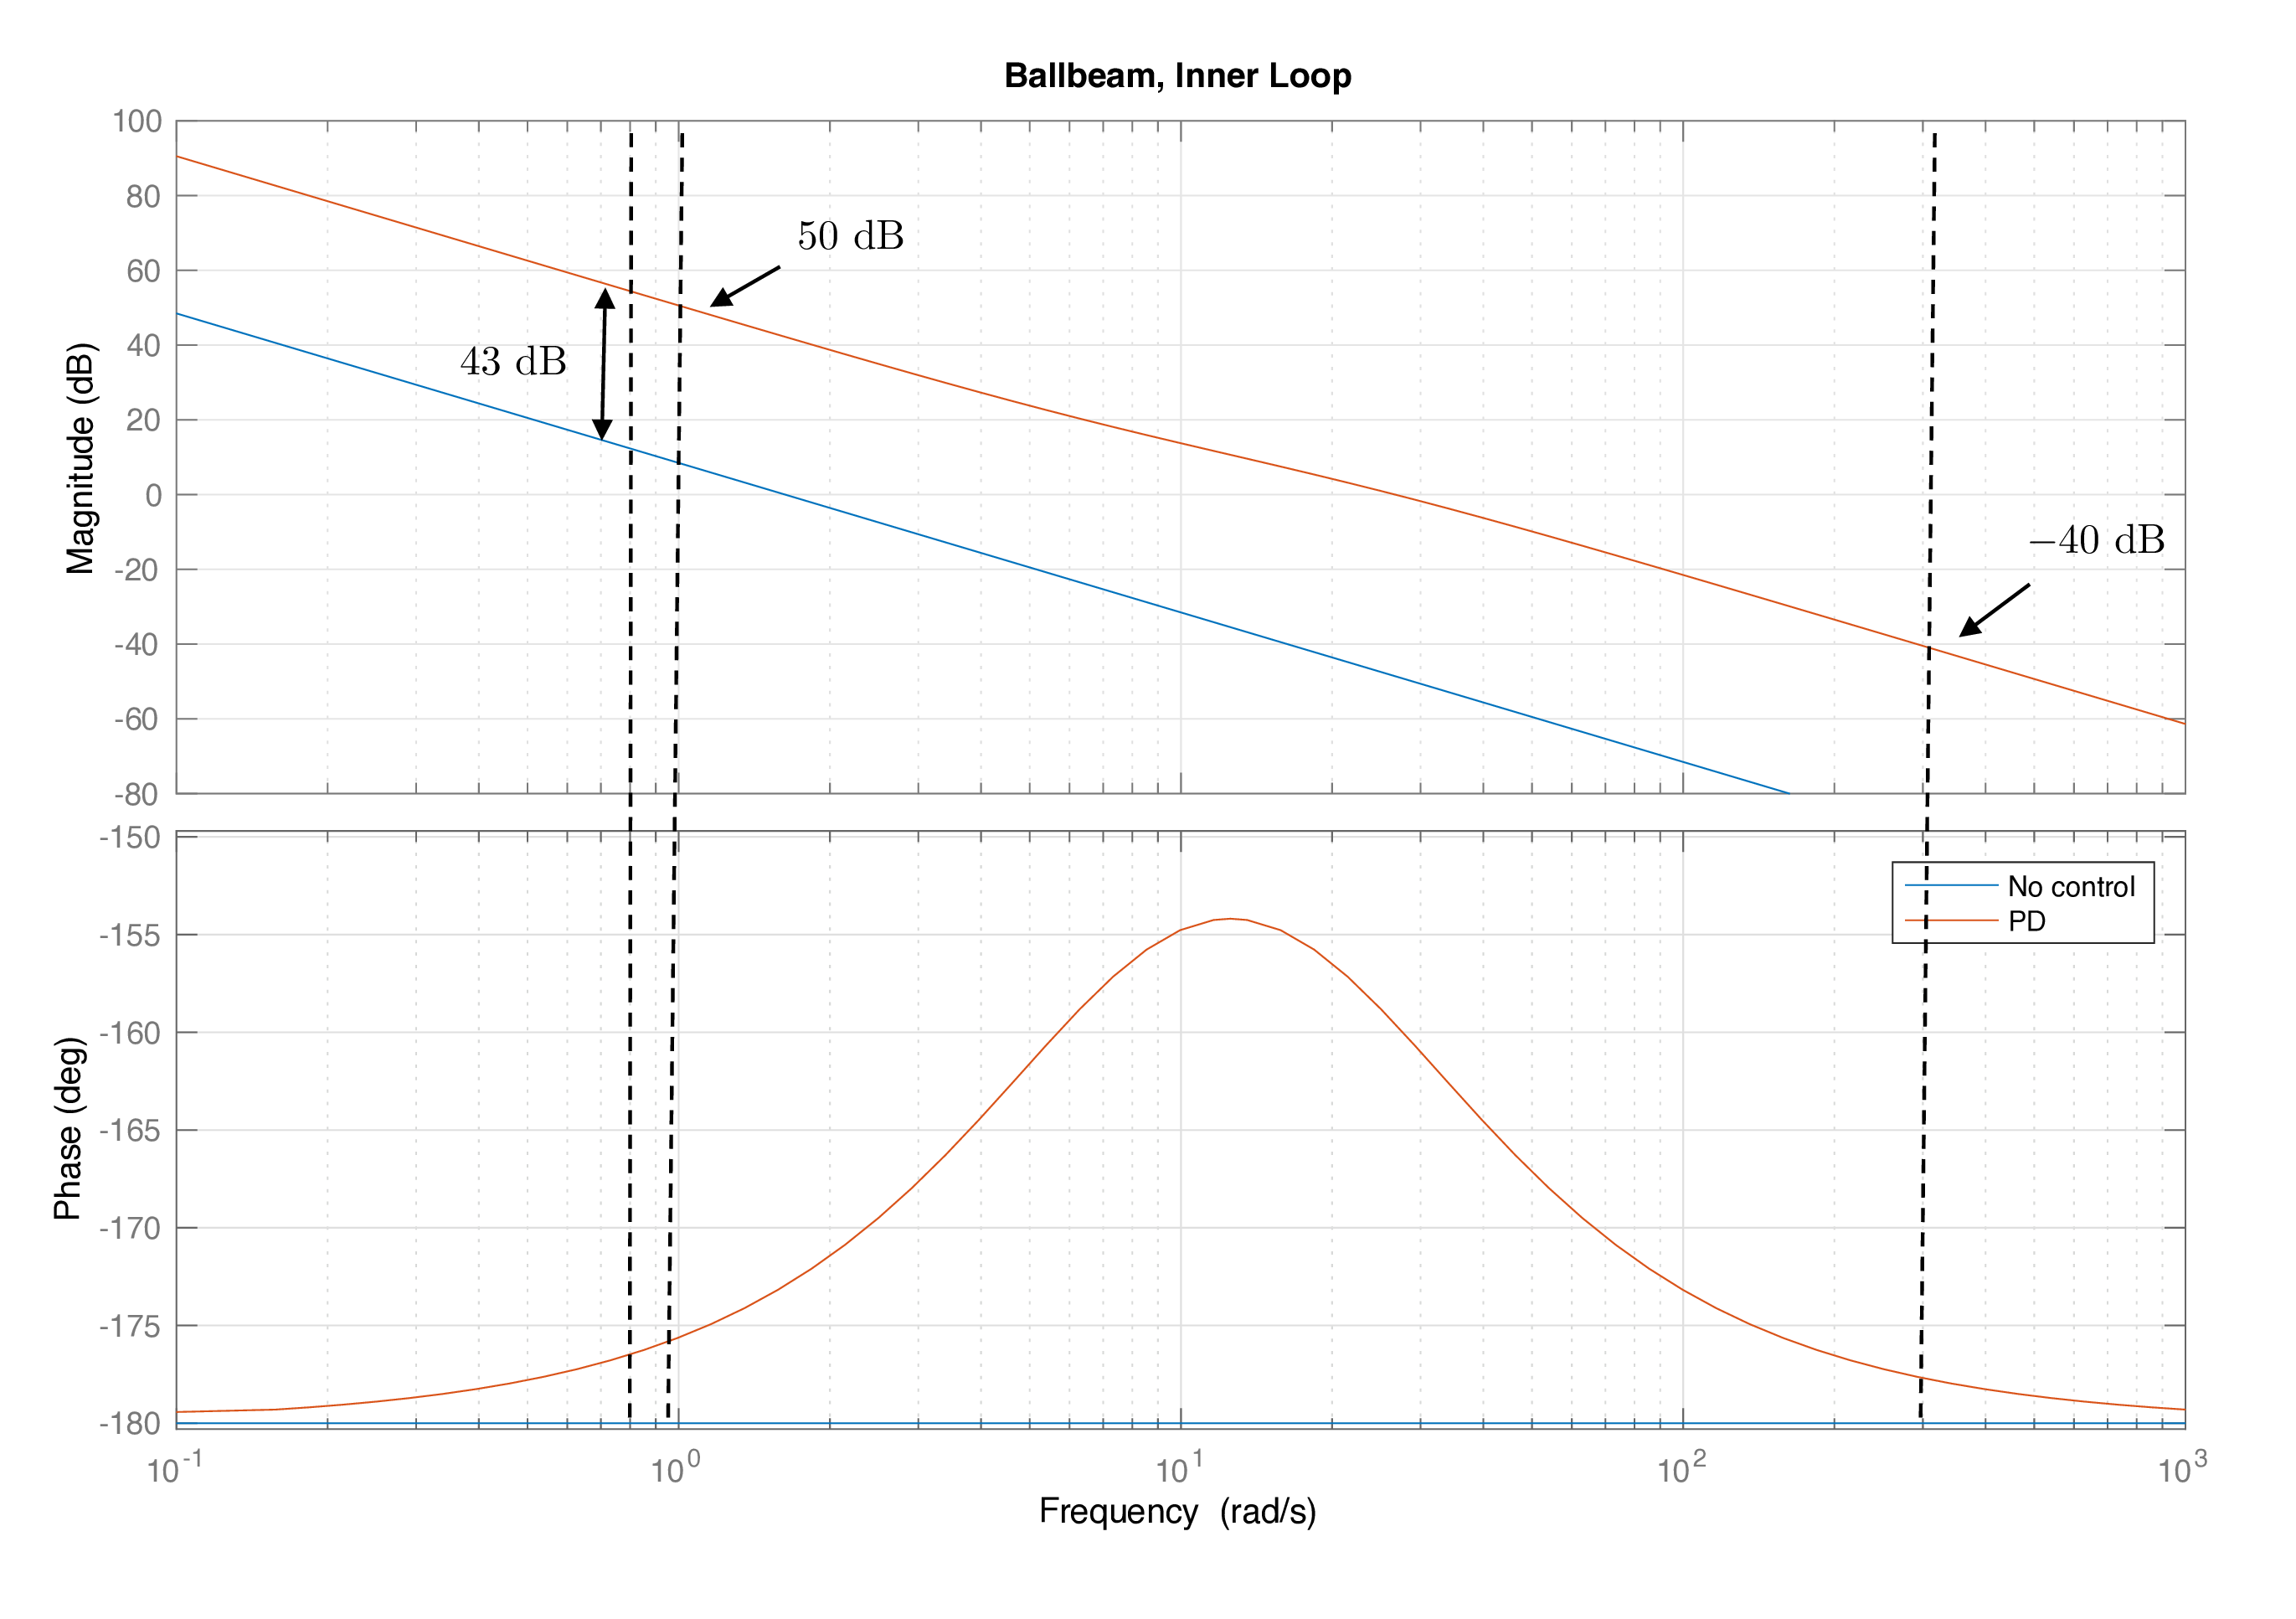
\includegraphics[width=0.95\textwidth]{6_design_studies/figures/hw_ballbeam_bode_specs_in.pdf}
   \caption{Bode plot for ball and beam inner loop, plant only, and under PD control.}
   \label{fig:hw_ballbeam_bode_specs_in}
\end{figure}


{\bf (a)} From Figure~\ref{fig:hw_ballbeam_bode_specs_in} we see that for $\omega<\omega_r=1$~rad/sec, the loop gain is greater than $B_r=50$~dB.  Therefore, the tracking error satisfies
\[
\abs{e(t)}\leq 10^{-50/20}\abs{r(t)} = 0.0032 \abs{r(t)},
\]
which implies that tracking accuracy is to within $0.32$\%.


{\bf (b)} From Figure~\ref{fig:hw_ballbeam_bode_specs_in} we see that for $\omega\leq\omega_{d_{in}}=0.8$~dB, the Bode magnitude plot satisfies 
\[
20\log_{10}\abs{P(j\omega)C(j\omega)}-20\log_{10}\abs{P(j\omega)} \geq B_{d_{in}}=43\text{~dB}.
\]  
Therefore, the contribution of the input disturbance to the error satisifies
\[
\abs{e(t)} \leq 10^{-43/20}\abs{d_{in}(t)} = 0.0071\abs{d_{in}(t)},
\]
which implies that $0.71$\% of the input disturbance shows up in the output $\theta$.

{\bf (c)} For $\omega\geq\omega_{no}=300$~rad/sec, we see from Figure~\ref{fig:hw_ballbeam_bode_specs_in} that $B_{no} = -40$~dB.  Therefore, $\gamma_n = 10^{-40/20} = 0.01$ which implies that $1$\% of the noise will show up in the output signal.


The Bode plot of the outer loop $P_{out}(s)$, and the loop gain with PD control $P_{in}(s)C_{PD}(s)$, and with  PID control $P_{in}(s)C_{PID}(s)$ are shown in Figure~\ref{fig:hw_ballbeam_bode_specs_out}.
\begin{figure}[H]
   \centering
   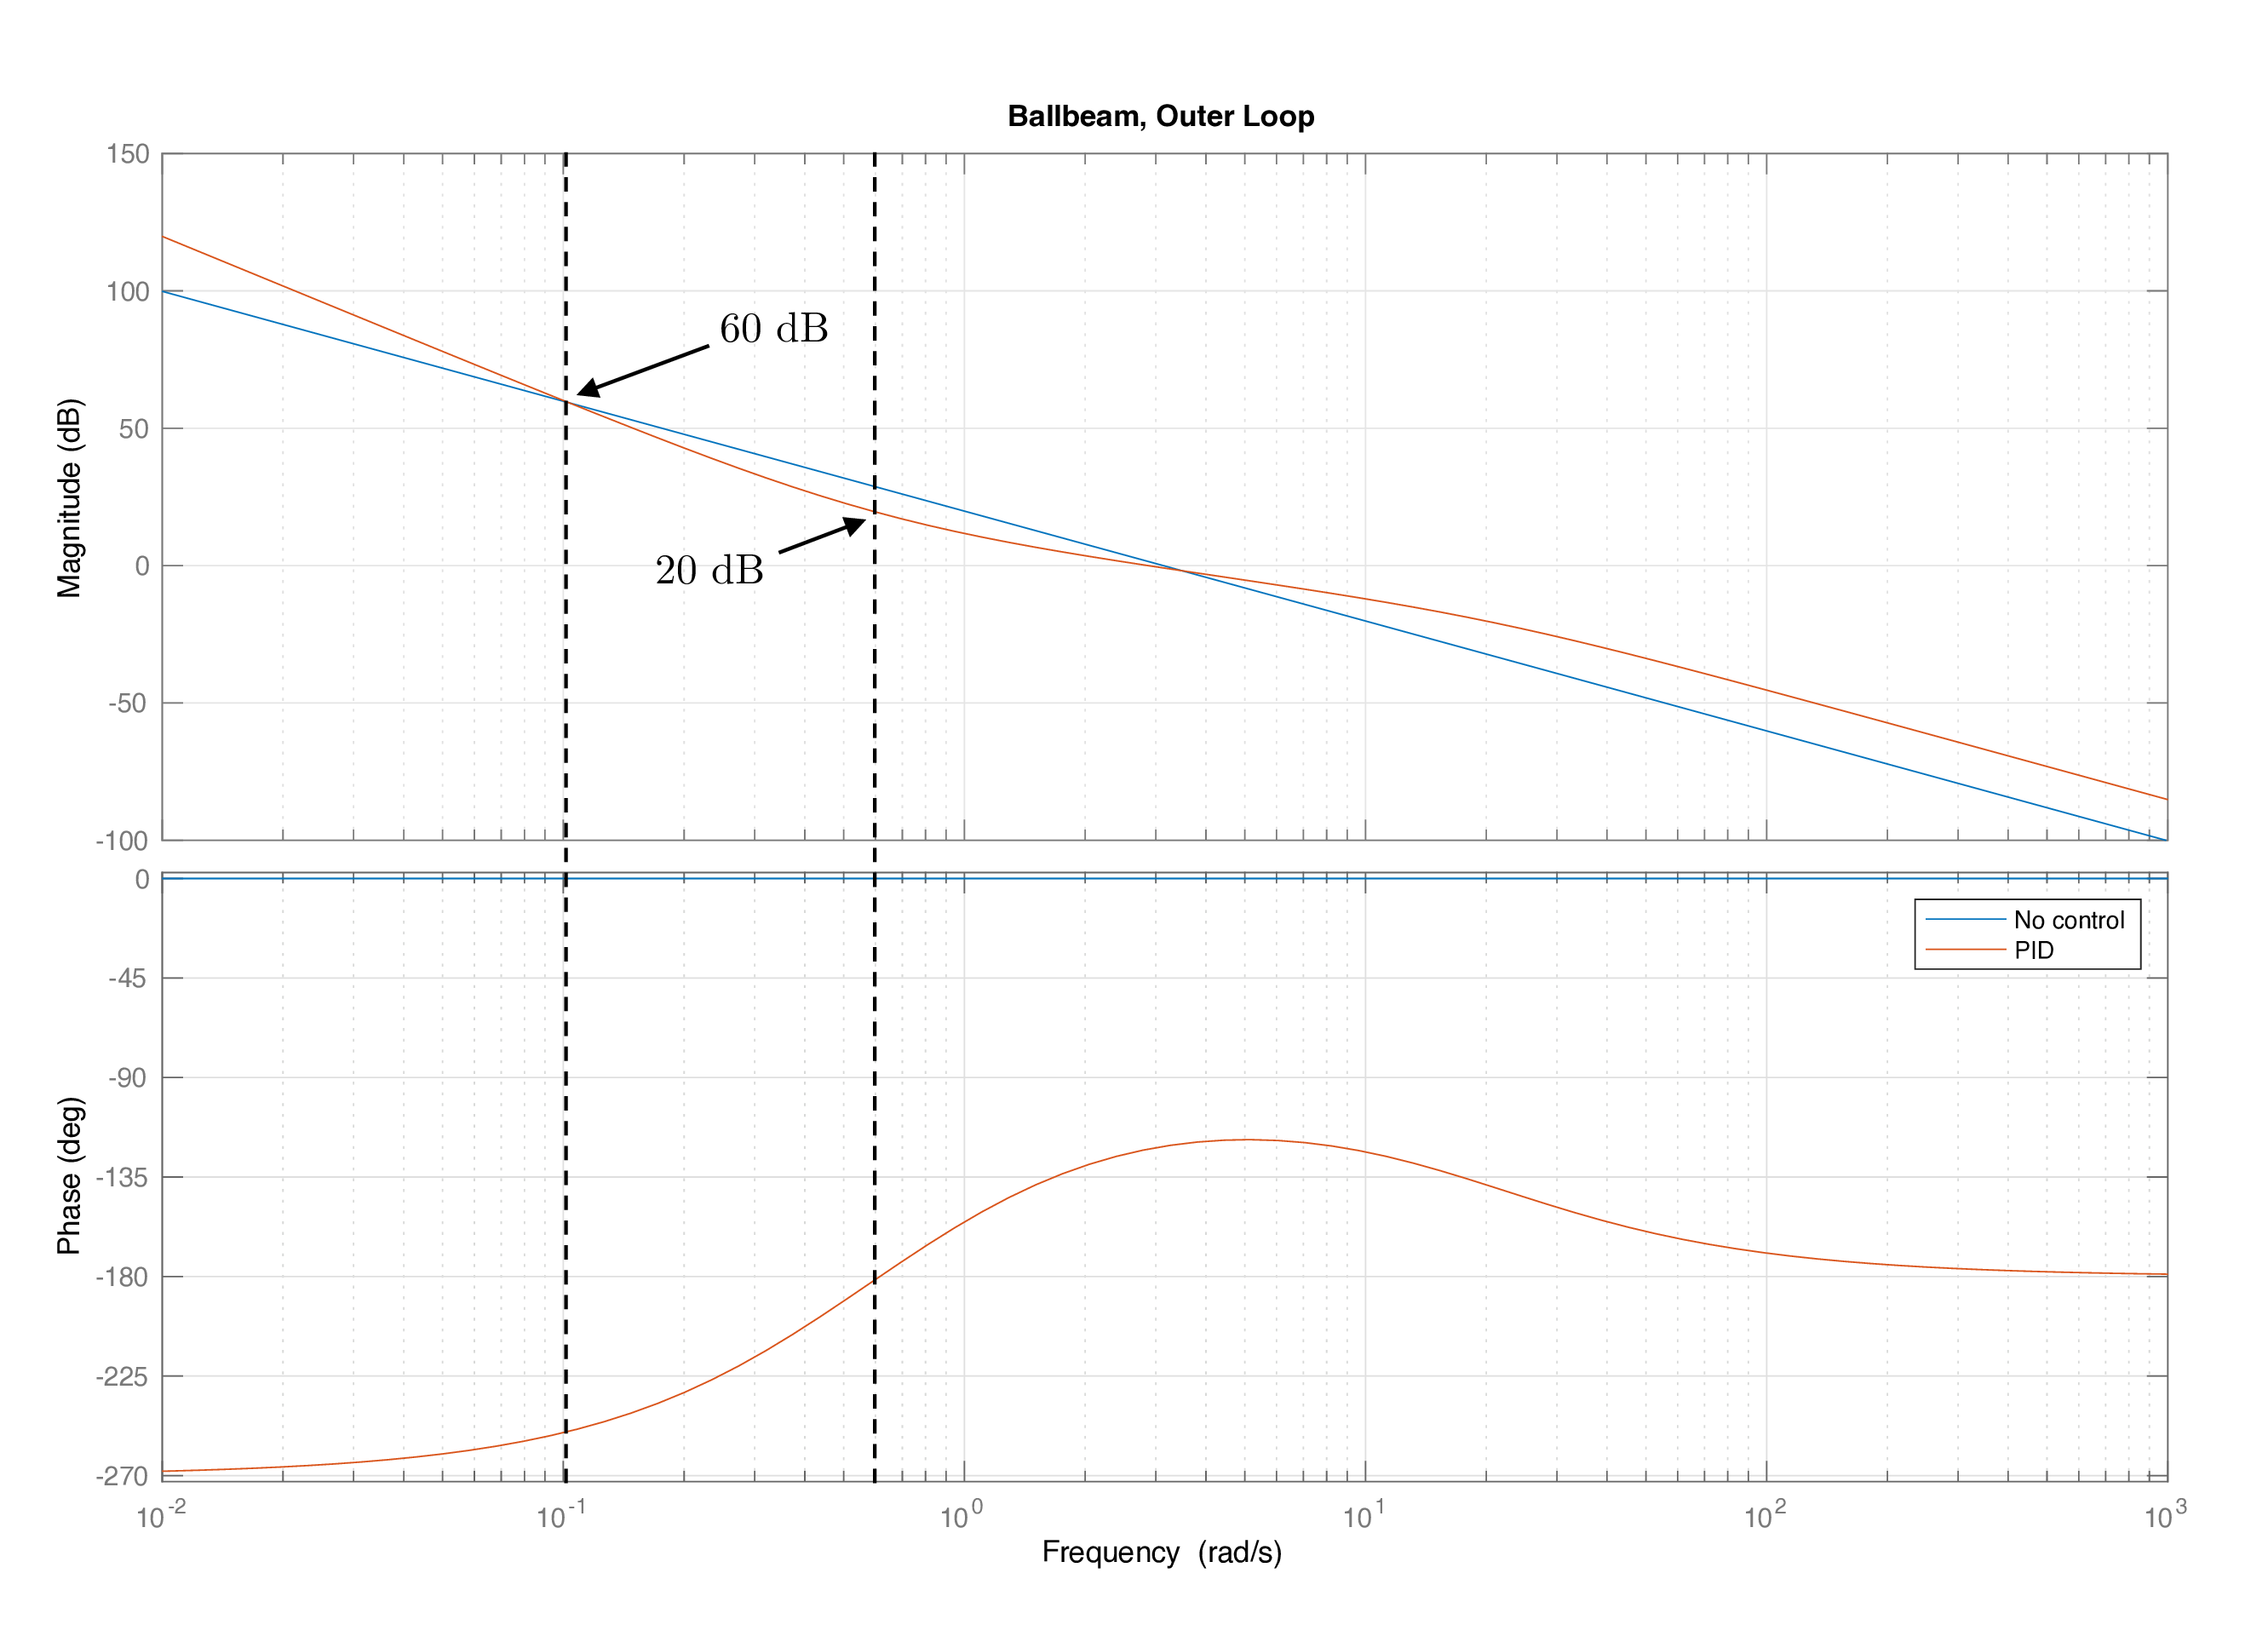
\includegraphics[width=0.95\textwidth]{6_design_studies/figures/hw_ballbeam_bode_specs_out.pdf}
   \caption{Bode plot for ball and beam outer loop, plant only, under PD control, and under PID control.}
   \label{fig:hw_ballbeam_bode_specs_out}
\end{figure}


{\bf (d)} For $\omega\leq\omega_{d_{out}}=0.1$~rad/sec, we see from Figure~\ref{fig:hw_ballbeam_bode_specs_out} that for  PID control $B_{d_{out}} = 60$~dB.  Therefore, $\gamma_{d_{in}} = 10^{-60/20} = 0.001$, which implies that $0.1$\% of the output disturbance will show up in the output signal.


{\bf (e)} At $\omega_0=0.6$~rad/sec, we see from Figure~\ref{fig:hw_ballbeam_bode_specs_out} that the loop gain is $20\log_{10} \abs{P(j\omega_0) C_{PD}(j\omega_0)} = 20$~dB.  Therefore, the tracking error will be
\[
\abs{e(t)}=\abs{\frac{1}{1+P(j\omega_0)C(j\omega_0)}}\cdot 2 \approx \abs{\frac{1}{P(j\omega_0)C(j\omega_0)}}\cdot 2 = \frac{2}{10^{20/20}} = 0.2.
\]

